%%%%%%%%%%%%%%%%%%%%%%%%%%%%%%%%%%%%%%%%%%%%%%%%%%%%%%%%%%%%%%%%%%%%%%%%%%%%%%%%%%
\begin{frame}[fragile]\frametitle{}
\begin{center}
{\Large Conclusions}
\end{center}
\end{frame}

%%%%%%%%%%%%%%%%%%%%%%%%%%%%%%%%%%%%%%%%%%%%%%%%%%%%%%%%%%%
\begin{frame}[fragile]\frametitle{So, What is RAG?}

\begin{itemize}
\item A new paradigm for generation tasks, combining retrieval and generation models.
\item Motivation: Overcoming limitations of pure generative models in factual consistency, efficiency, and diversity.
\item Impact: Improved performance in text summarization, question answering, and other NLP tasks.
\end{itemize}	



		\begin{center}
		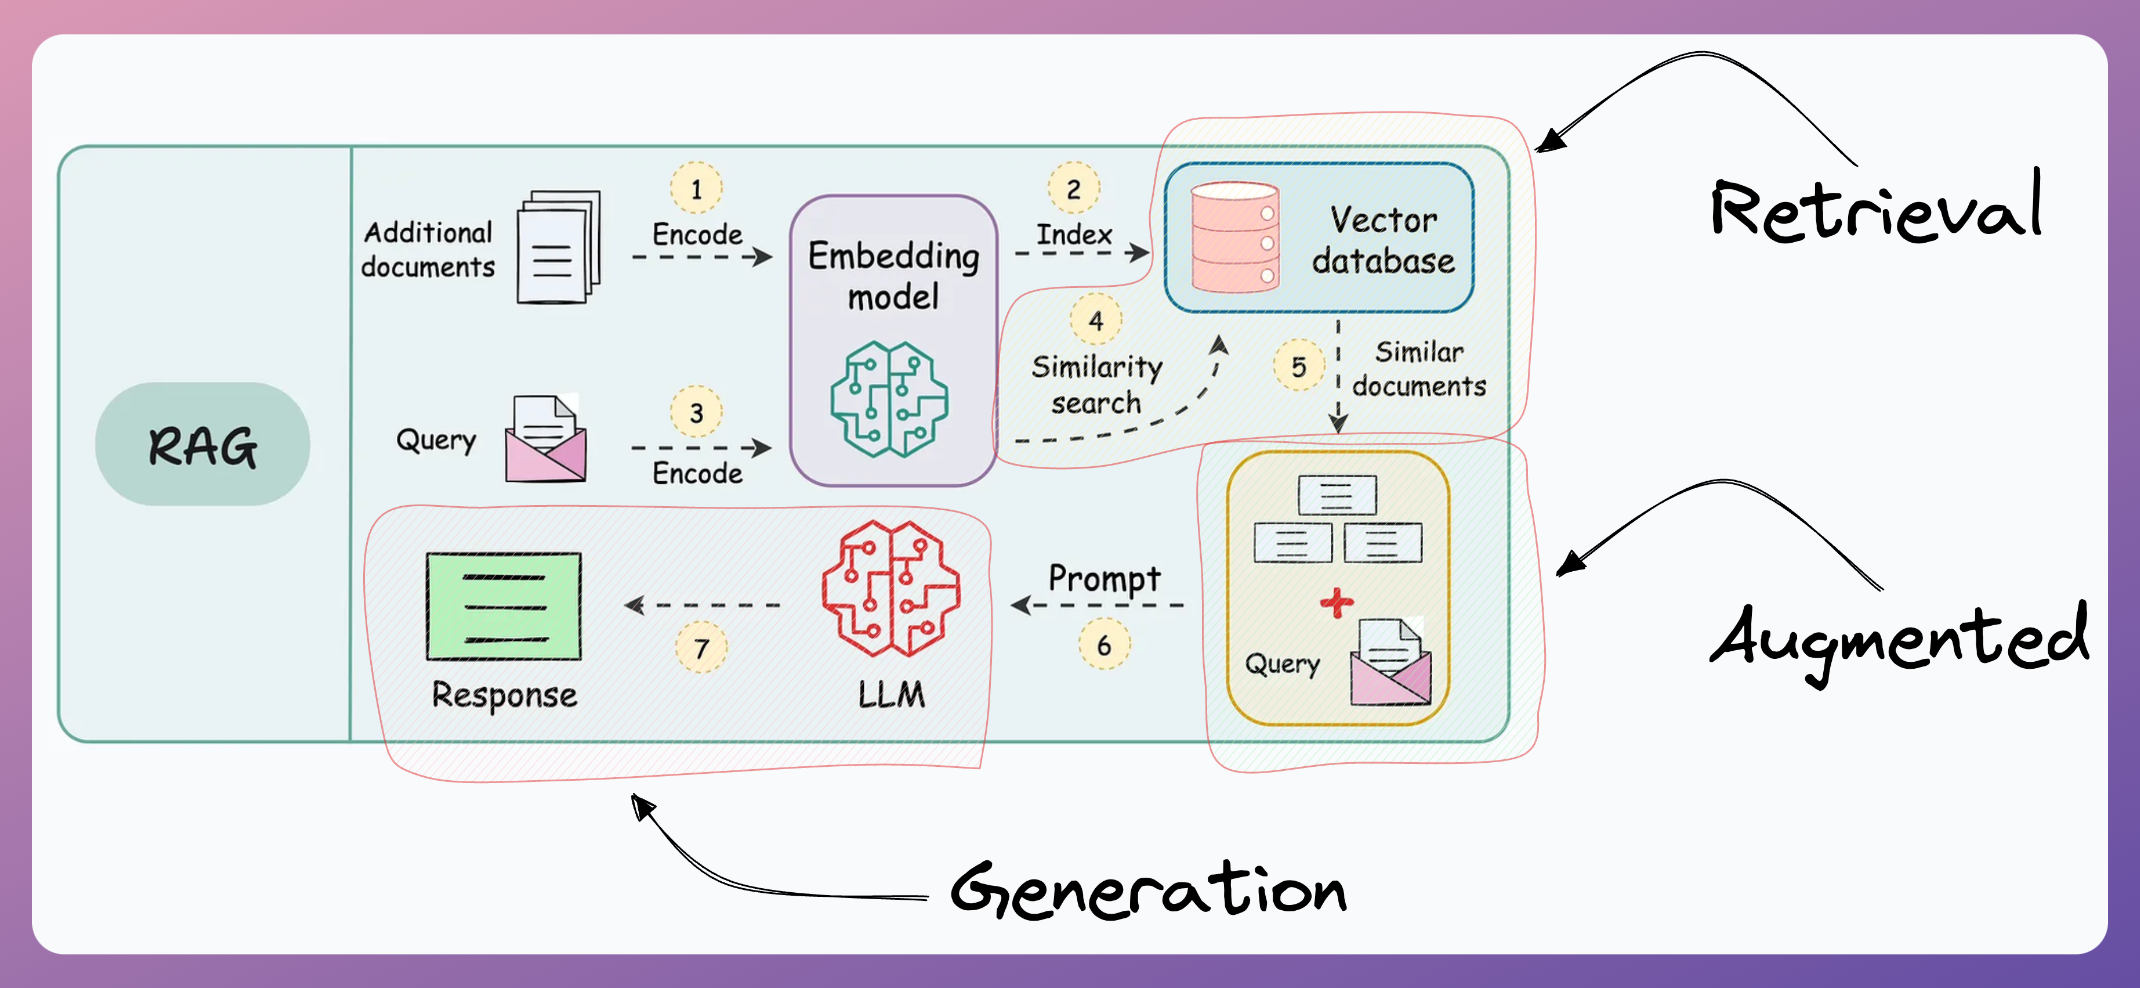
\includegraphics[width=0.8\linewidth,keepaspectratio]{rag48}
		
		
		\end{center}

{\tiny (Ref: A Crash Course on Building RAG Systems -Daily Dose)}


\end{frame}

%%%%%%%%%%%%%%%%%%%%%%%%%%%%%%%%%%%%%%%%%%%%%%%%%%%%%%%%%%%
\begin{frame}[fragile]\frametitle{RAG Workflow}



		\begin{center}
		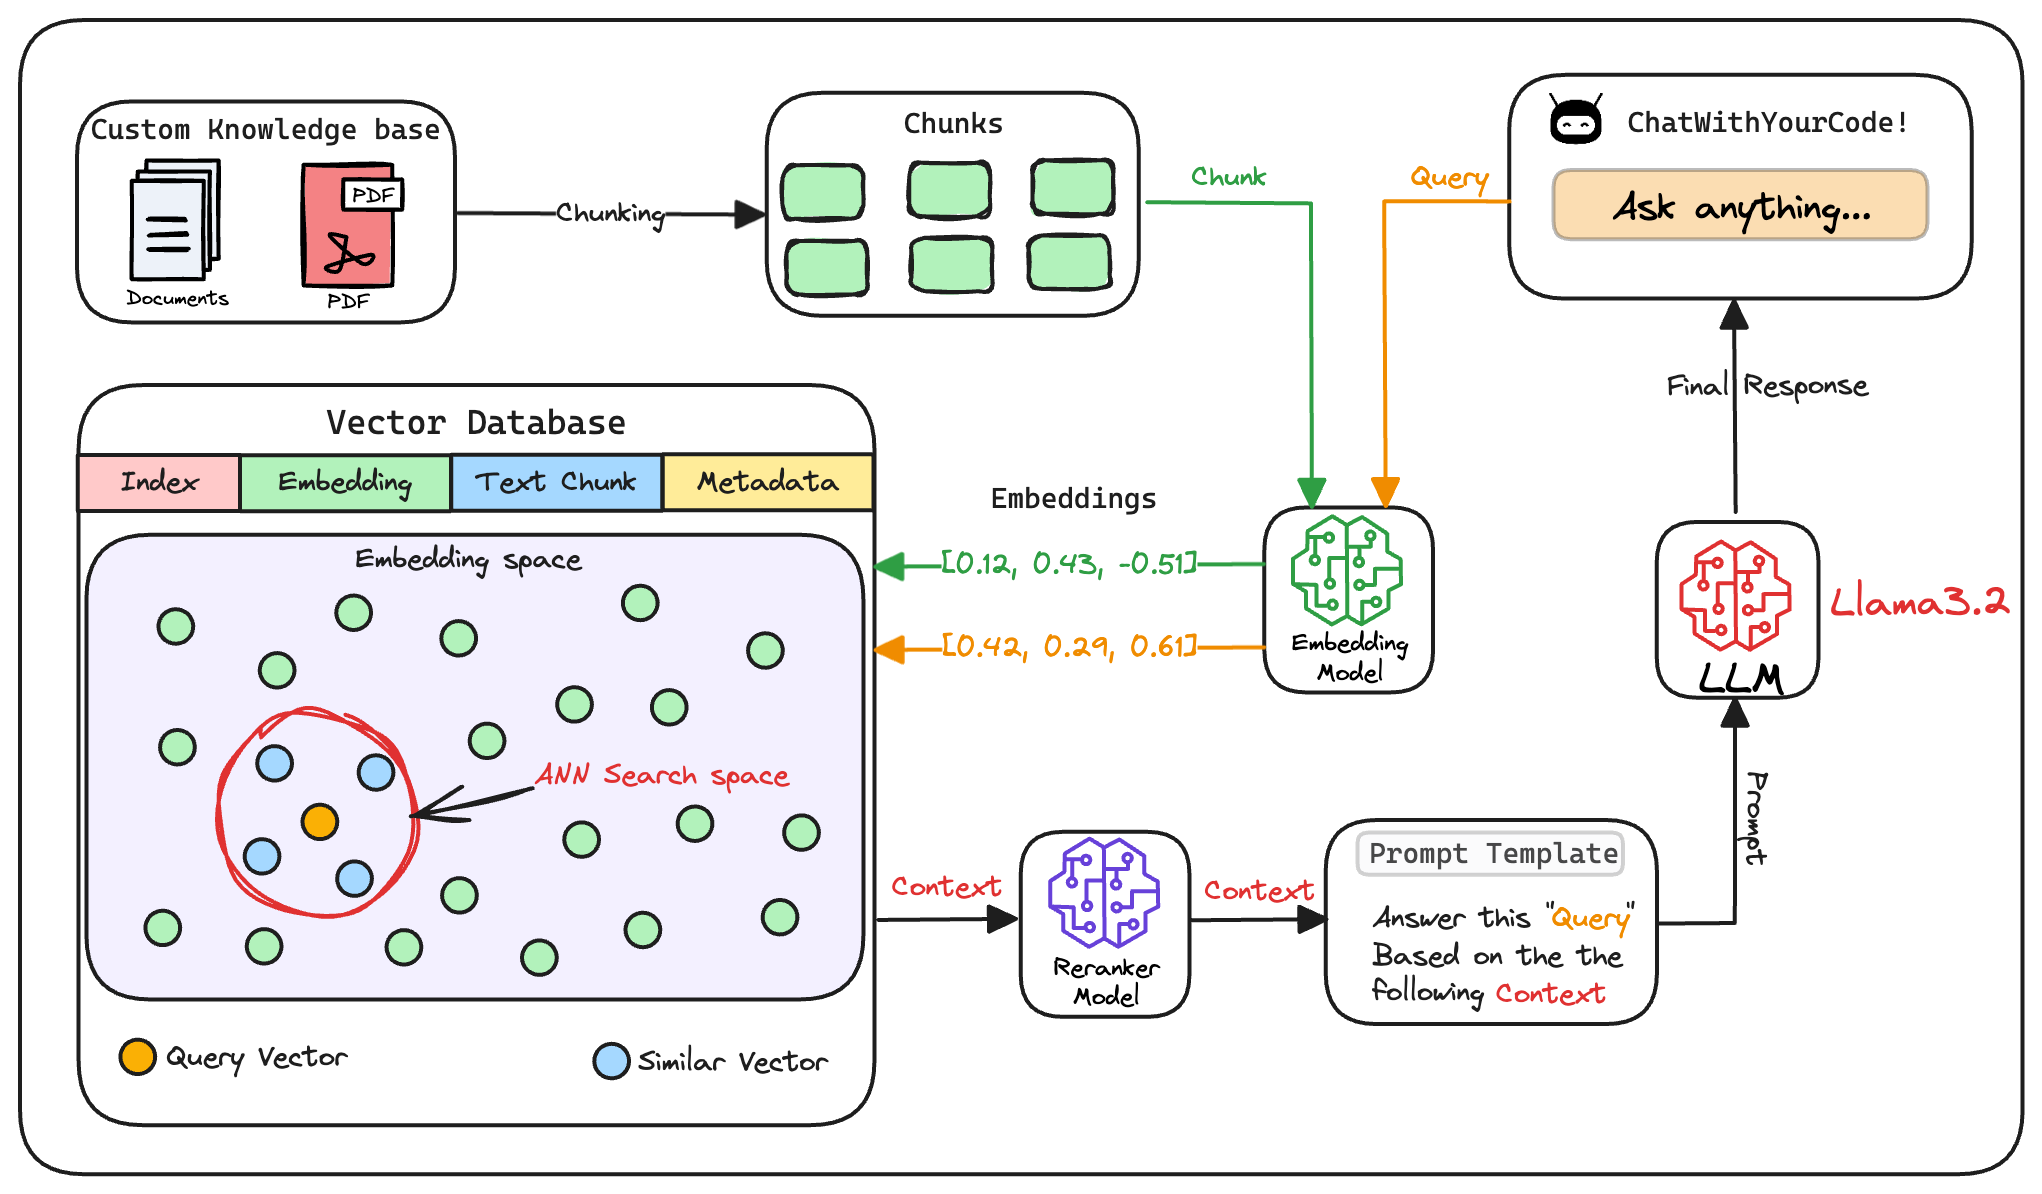
\includegraphics[width=0.8\linewidth,keepaspectratio]{rag49}
		
		
		\end{center}

{\tiny (Ref: A Crash Course on Building RAG Systems -Daily Dose)}


\end{frame}



%%%%%%%%%%%%%%%%%%%%%%%%%%%%%%%%%%%%%%%%%%%%%%%%%%%%%%%%%%%
\begin{frame}[fragile]\frametitle{RAG Architecture}


		\begin{center}
		\includegraphics[width=0.5\linewidth,keepaspectratio]{chatgpt47}
		\end{center}

{\tiny (Ref: Overview of Large Language Models - Aman AI)}

\end{frame}


%%%%%%%%%%%%%%%%%%%%%%%%%%%%%%%%%%%%%%%%%%%%%%%%%%%%%%%%%%%
\begin{frame}[fragile]\frametitle{RAG Architecture}

\begin{itemize}
  \item \textbf{Powerful Enhancement:}
    \begin{itemize}
      \item RAG provides additional memory and context.
      \item Increases confidence in LLM responses.
    \end{itemize}

  \item \textbf{Architecture:}
    \begin{itemize}
      \item Two essential pipelines for an effective RAG system.
    \end{itemize}
  
  \item \textbf{Indexing Pipeline:}
    \begin{itemize}
      \item Retrieves knowledge from diverse sources.
      \item Enables loading, splitting, and embedding creation for offline use.
      \item Can be on-the-fly for lower volume and single-use scenarios.
    \end{itemize}

  \item \textbf{Generation Pipeline:}
    \begin{itemize}
      \item Retriever fetches information from the knowledge base.
      \item Retrieved data augments user prompt and is sent to the LLM.
      \item LLM generates text and sends the response back to the user.
    \end{itemize}

  \item \textbf{Evaluation Pipeline:}
    \begin{itemize}
      \item Optional pipeline for assessing groundedness and relevance of responses.
    \end{itemize}
\end{itemize}

{\tiny (Ref: RAG Architecture -Abhinav  Kimothi)}

\end{frame}

%%%%%%%%%%%%%%%%%%%%%%%%%%%%%%%%%%%%%%%%%%%%%%%%%%%%%%%%%%%
\begin{frame}[fragile]\frametitle{The Core RAG Bottleneck}
      \begin{itemize}
        \item 90\% of RAG systems fail due to poor retrieval.
        \item Better LLMs do not fix bad retrieval.
        \item Naive RAG: Chunk, embed, retrieve top\_k — too simplistic.
        \item Poor retrieval causes hallucinations, omissions, and vague outputs.
        \item Quality of generation depends on quality of retrieved context.
      \end{itemize}
\end{frame}

%%%%%%%%%%%%%%%%%%%%%%%%%%%%%%%%%%%%%%%%%%%%%%%%%%%%%%%%%%%
\begin{frame}[fragile]\frametitle{Step 1: Fix the Basics}
      \begin{itemize}
        \item Use dynamic chunking that respects document structure.
        \item Tune chunk size to avoid loss or fragmentation.
        \item Apply metadata filtering to narrow semantic scope.
        \item Combine vector search with keyword filters (hybrid).
      \end{itemize}
\end{frame}

%%%%%%%%%%%%%%%%%%%%%%%%%%%%%%%%%%%%%%%%%%%%%%%%%%%%%%%%%%%
\begin{frame}[fragile]\frametitle{Step 2: Advanced Retrieval Techniques}
      \begin{itemize}
        \item Apply re-ranking (learned or rule-based).
        \item Use small-to-big retrieval: start with sentences.
        \item Employ recursive retrieval methods like LlamaIndex.
        \item Use multi-hop and agentic retrieval for complex queries.
      \end{itemize}
\end{frame}

%%%%%%%%%%%%%%%%%%%%%%%%%%%%%%%%%%%%%%%%%%%%%%%%%%%%%%%%%%%
\begin{frame}[fragile]\frametitle{Step 3: Evaluate or Die Trying}
      \begin{itemize}
        \item Don’t iterate blindly — evaluate systematically.
        \item Use end-to-end evaluation with ground truths or feedback.
        \item Run component-level evals using MRR, NDCG, success@k.
      \end{itemize}
\end{frame}

%%%%%%%%%%%%%%%%%%%%%%%%%%%%%%%%%%%%%%%%%%%%%%%%%%%%%%%%%%%
\begin{frame}[fragile]\frametitle{Step 4: Fine-Tuning — A Last Resort}
      \begin{itemize}
        \item Fine-tune only if domain is highly specific or LLM is weak.
        \item Ensure retrieval and prompting are fully optimized first.
        \item Be aware of added cost, latency, and system complexity.
      \end{itemize}
\end{frame}



%%%%%%%%%%%%%%%%%%%%%%%%%%%%%%%%%%%%%%%%%%%%%%%%%%%%%%%%%%%
\begin{frame}[fragile]\frametitle{Pros and Cons of RAG}

\begin{itemize}
\item Pros: Improved factual accuracy, diversity, and efficiency compared to pure generation.
\item Cons: Increased complexity, potential bias introduced by the retrieval component, and dependency on external corpus quality.
\end{itemize}	

\end{frame}

%%%%%%%%%%%%%%%%%%%%%%%%%%%%%%%%%%%%%%%%%%%%%%%%%%%%%%%%%%%
\begin{frame}[fragile]\frametitle{Challenges and Future Directions}

\begin{itemize}
\item Bias Mitigation: Addressing potential biases introduced by the retrieval component.
\item Domain Adaptation: Adapting RAG models to specific domains with limited training data.
\item Interpretability Enhancement: Understanding the reasoning behind generated outputs for better model debugging.
\end{itemize}	

\end{frame}